\documentclass{standalone}

\usepackage{tikz}
\usetikzlibrary{calc}
\usetikzlibrary{math}


\def\memory#1#2#3#4{
  \begin{scope}
    \def\names{#2}
    \def\values{{#3}}

    \node at ($ #1 + (1, -0.2) $) {\tiny #4};
    \draw[fill=gray!10] #1 rectangle ++(2, 2.75);

    \foreach \name [count=\i] in \names
    {
      \tikzmath{\val= \values[\i-1];}

      \node at ($ #1 + (0.4, -0.5 + \i * 1.25) $) {\name};
      \draw[draw=black, fill=white] ($ #1 + (0.75, -1 + \i * 1.25) $) rectangle ++(1, 1)
                        node[pos=.5] {\val};
    }
  \end{scope}
}

\begin{document}
  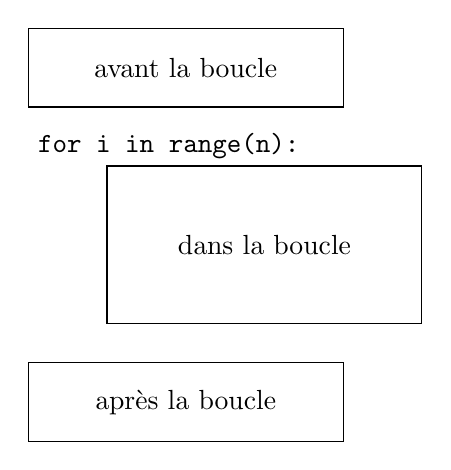
\begin{tikzpicture}
    \draw[draw=black] (0, 4.25) rectangle ++(4, 1) node[pos=.5] {%
      avant la boucle
    };

    \node[anchor=west] at (0, 3.75) {\texttt{for i in range(n):}};

    \draw[draw=black] (1, 1.5) rectangle ++(4, 2) node[pos=.5] {%
      dans la boucle
    };

    \draw[draw=black] (0, 0) rectangle ++(4, 1) node[pos=.5] {%
      apr\`es la boucle
    };
  \end{tikzpicture}
\end{document}
